\section{Filtros}
En las figuras \ref{fig:2017} y \ref{fig:2020} se grafica la relación entre la energía y el valor de $S_{38}$ en forma de log-log, ya que para el cálculo de la energía se utiliza la relación $E=A(S_{38})^B$. Las correcciones del clima en este análisis no son importantes porque 
se estudia la relación entre energía y la señal en los tanques. Es posible que utilizando los eventos medidos con los FD, los  parámetros A y B cambien si usamos los eventos híbridos, pero no es lo que estamos viendo acá. Los valores utilizados son tal cual aparecen en el conjunto de datos de la Colaboración Pierre Auger. Para seleccionar los eventos se usaron los siguientes filtros:

\begin{itemize}
	\item Number of selected Stations $>2$ (Columna 2) 
	\item Estimation and Reconstruction compatibles $>0$  (Columna 22)  
	\item Is T5 $>0$  (Columna 23)  
	\item Número de vecinos $>5$  (Columna 43) 
	\item Containment Flag $>0$  (Columna 44)  
\end{itemize}

Además de considerar los eventos coincidentes entre ambos datasets. En total se obtiene 6\,902\,211 de eventos, entre el 1 de Julio del 2013 12:01:08 GMT \footnote{$1372680068$ UTC} y el 26 de Junio del 2017 23:58:37 GMT \footnote{$1498521517$ UTC}.


En la Fig.\,\ref{fig:2017} se observa que los eventos caen sobre una recta. Para energías menores a $1 $EeV se observa que la recta no está bien definida, esto puede deberse a cuestiones de redondeo durante el cálculo de energía. En la Fig.\,\ref{fig:2020} en cambio se observa  dos rectas, con pendientes y valores en el origen distintas, lo cual no es de esperarse ya que puede decirse que existen dos calibraciones entre energía y $S_{38}$. 

Algo que cabe resaltar de que los eventos que generan esta recta de calibración adicional, son de un rango de tiempo en particular, a partir del 1 de Enero de 2014 12:00:00 GMT \footnote{ 1388577600 UTC}. En la siguiente sección estudiaremos el set de datos antes y después esta fecha.


\begin{figure}[H]
	\centering
	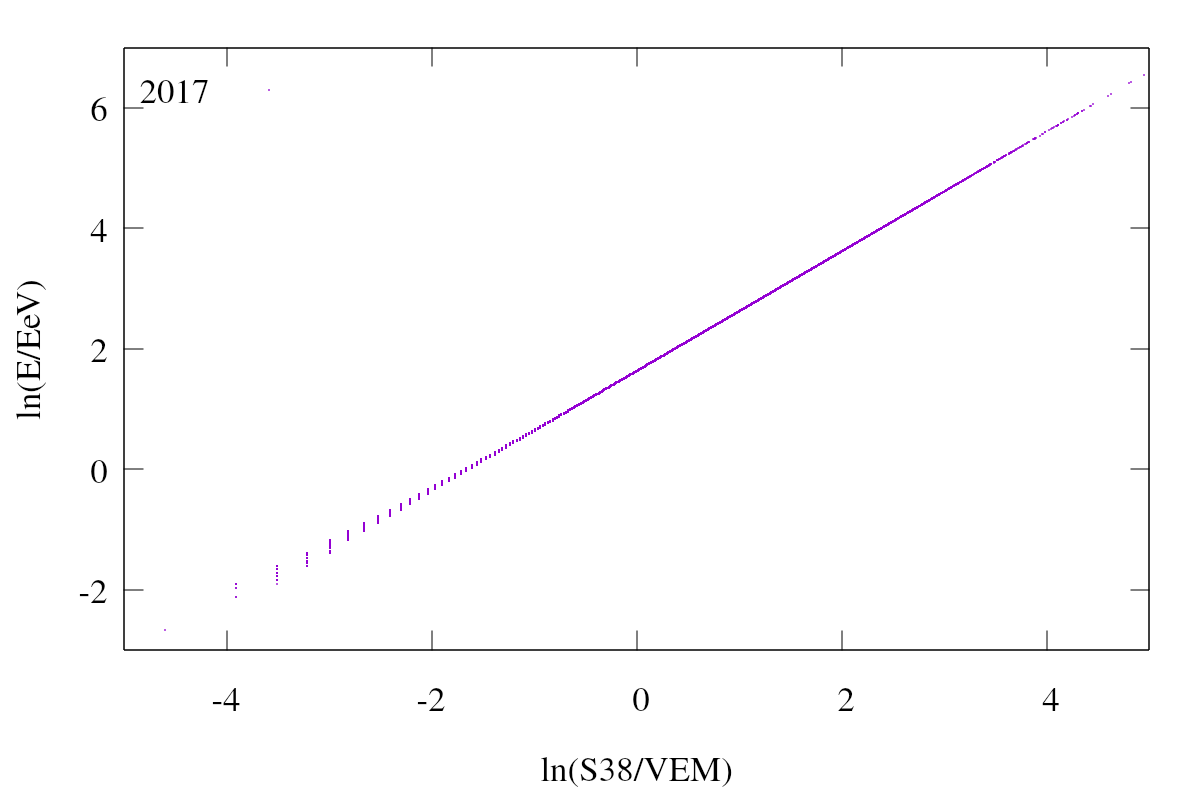
\includegraphics[width=0.5\textwidth]{curva_calibracion_all_2017.png}
	\caption{Reconstrucción de los eventos para la versión anterior del algoritmo de CDAS.}
	\label{fig:2017}
\end{figure}


\begin{figure}[H]
	\centering
	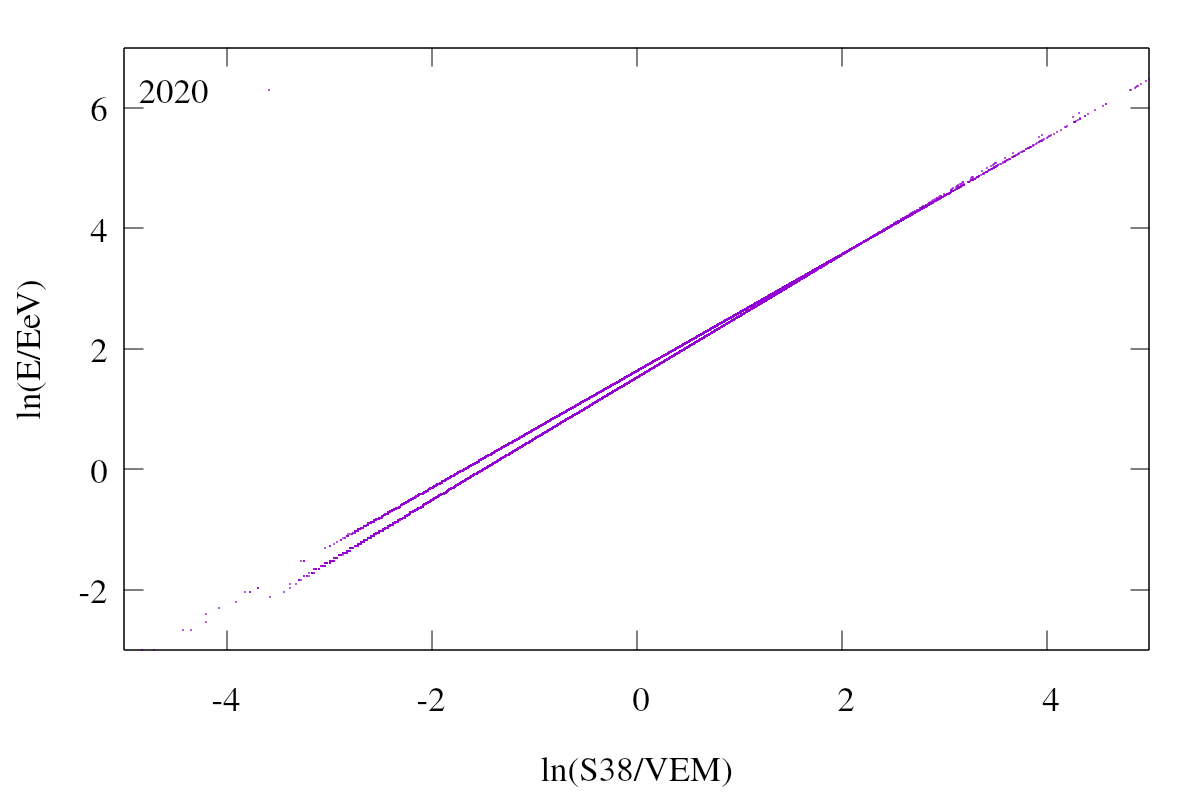
\includegraphics[width=0.5\textwidth]{curva_calibracion_all_2020.png}
	\caption{Reconstrucción de los eventos del archivo subido a la página en el año 2020. Se observan dos rectas superpuestas.}
	\label{fig:2020}
\end{figure}


\section{Para los eventos entre 1 EeV y 2 EeV}

Para los siguientes gráficos, se consideran solamente los eventos coincidentes con energías en el rango de energías 1 EeV - 2 EeV, porque son los que estamos usando para estudiar las anisotropías. 

Como se veía en la sección anterior y se observa nuevamente en las Figs.\,\ref{fig:solamente_2013} y \ref{fig:despues_2013}, existen 3 rectas de calibración, una en el archivo viejo o dos en el nuevo. El cambio en los parámetros A y B se realizan en la colaboración, y no se espera que cambien tanto en cada actualización, por eso podemos usar  la recta del archivo viejo como referencia.

En la Fig.\,\ref{fig:solamente_2013}, se observa que la recta del archivo 2020 durante el 2013 tiene un valor distinto en el origen y una pendiente distinta. En la Fig.\,\ref{fig:despues_2013}, para los eventos después del 2013, los utilizados en la tesis, se superpone bien con la calibración vieja salvo una diferencia en la pendiente. Los valores obtenidos en los ajustes son los siguientes:


\begin{table}[H]
\centering
\begin{tabular}{l|l|l|}
\cline{2-3}
                                 & \multicolumn{2}{c|}{Durante el 2013}                                   \\ \hline
\multicolumn{1}{|l|}{Parámetros} & \multicolumn{1}{c|}{Archivo 2017} & \multicolumn{1}{c|}{Archivo 2020}  \\ \hline
\multicolumn{1}{|l|}{B}          & $0.993 \pm 0.002$                 & $1.0176\pm 0.0004$                 \\ \hline
\multicolumn{1}{|l|}{ln(A)}      & $1.6342 \pm 0.0006$               & $1.5242\pm 0.0001$                 \\ \hline
\multicolumn{1}{|l|}{A}          & $5.125\pm 0.002$                  & $4.5914\pm 0.0003$                 \\ \hline
\end{tabular}
\caption{Tabla con los ajustes obtenidos durante el año 2013}
\end{table}

\begin{table}[H]
\centering
\begin{tabular}{l|l|l|}
\cline{2-3}
                                 & \multicolumn{2}{c|}{Después del 2013}                                 \\ \hline
\multicolumn{1}{|l|}{Parámetros} & \multicolumn{1}{c|}{Archivo 2017} & \multicolumn{1}{c|}{Archivo 2020} \\ \hline
\multicolumn{1}{|l|}{B}          & $0.9915 \pm 0.0008 $              & $0.9694 \pm 0.0002$               \\ \hline
\multicolumn{1}{|l|}{ln(A)}      & $1.6345 \pm 0.0002$               & $1.6326 \pm 0.0001$               \\ \hline
\multicolumn{1}{|l|}{A}          & $5.1268 \pm 0.0006$               & $5.1172 \pm 0.0003$               \\ \hline
\end{tabular}
\caption{Tabla con los ajustes obtenidos para eventos posteriores al 2013}
\end{table}


\begin{figure}[H]
	\centering
	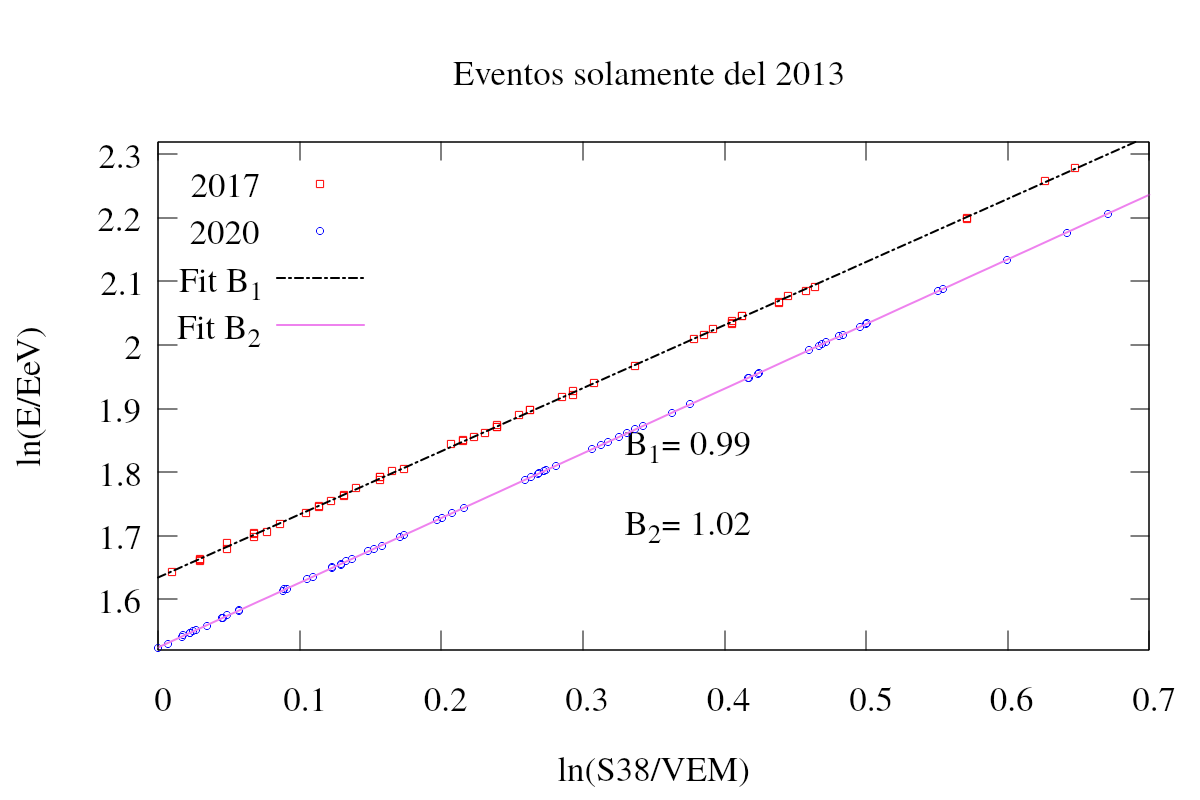
\includegraphics[width=0.5\textwidth]{curva_calibracion_solamente_2013.png}
	\caption{Eventos durante el 2013}
	\label{fig:solamente_2013}
\end{figure}



\begin{figure}[H]
	\centering
	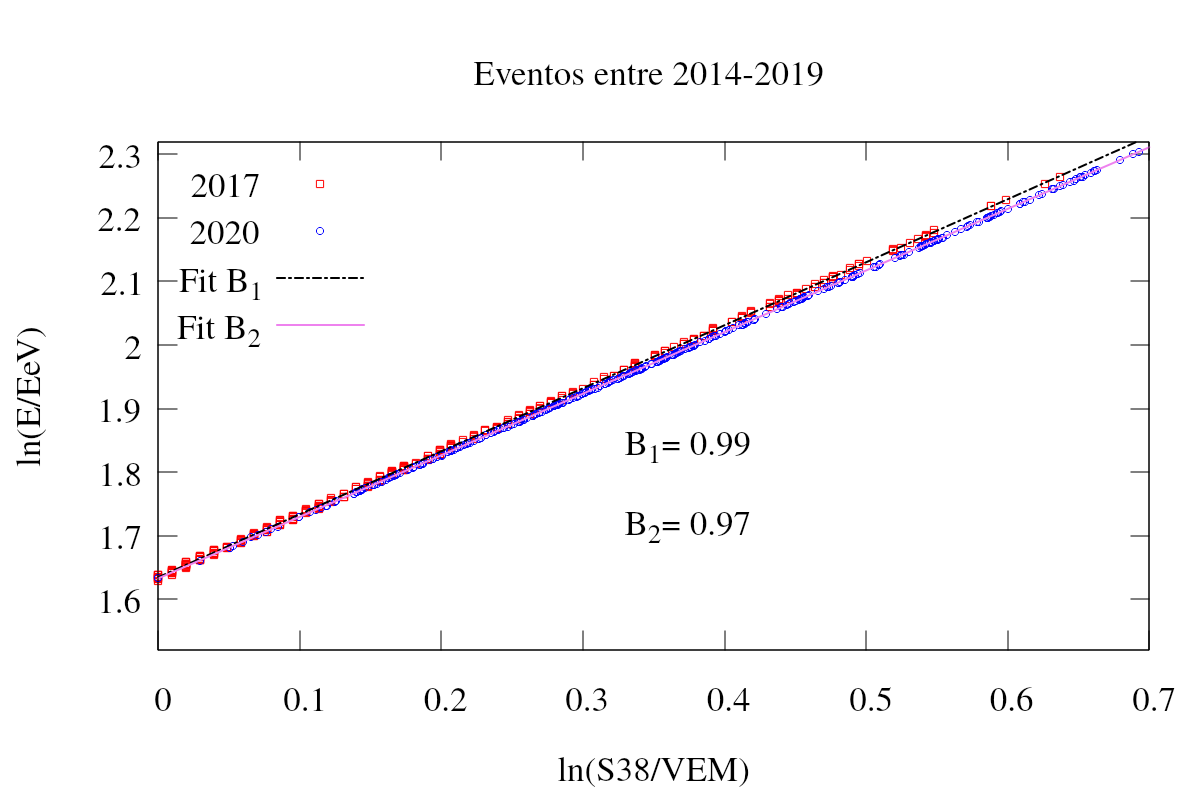
\includegraphics[width=0.5\textwidth]{curva_calibracion_comparando_2014-2020.png}
	\caption{Eventos después del 2013. Estos son los eventos considerados para los análisis de la tesis.}
	\label{fig:despues_2013}
\end{figure}